\documentclass{article}

% Gives us lovely headers
\usepackage{fancyhdr}
% For pretty pictures
\usepackage{graphicx}
% Means you don't have to put \\ to start a new line.
\usepackage[parfill]{parskip}
% For line brakes in tables
\usepackage{tabularx}
% For the split environment
\usepackage{amsmath}
% For tabs in verbatim and the listings environment
\usepackage{moreverb}
% Gives us bigger margins on the right (and smaller on the left) for the margin
% paragraphs
\usepackage[left=2cm,
			top=3cm,
			right=5cm,
			bottom=3cm,
			marginparwidth=4cm,
			marginparsep=3mm]{geometry}

% Means that I don't have to type \marginpar{\raggedright \scriptsize every 
% time I want a margin paragraph
\makeatletter
\renewcommand{\@marginparreset}{%
  \reset@font\scriptsize
  \raggedright
  \@setminipage
}
\makeatother

\begin{document}
% Meta
\author{Todd Davies}
\title{COMP12111 notes}
\rhead{COMP12111 notes}
\chead{}

\maketitle

{\small Note, extra space has been allocated for the right hand margin to allow
for more extensive margin notes. Also, it gives you space to make your own
annotations and perhaps try some problems of your own.}

\tableofcontents
\newpage

\section*{Introduction}

Unlike many of the courses, the university supplied notes for this course are of
a very high quality. This is especially true of the notes covering the first
half of the course (weeks one through six). In light of this, I've decided not
to write notes on the first half, but concentrate solely on the second half of
the course. However, it is likely that I will produce other resources such as
summary notes or flashcards for the whole of the course.

\section{The three box model}

The three box model describes the classic model of a computer. The three boxes
consist of the CPU, the memory and I/O.

\begin{figure}[ht!]
	\centering
	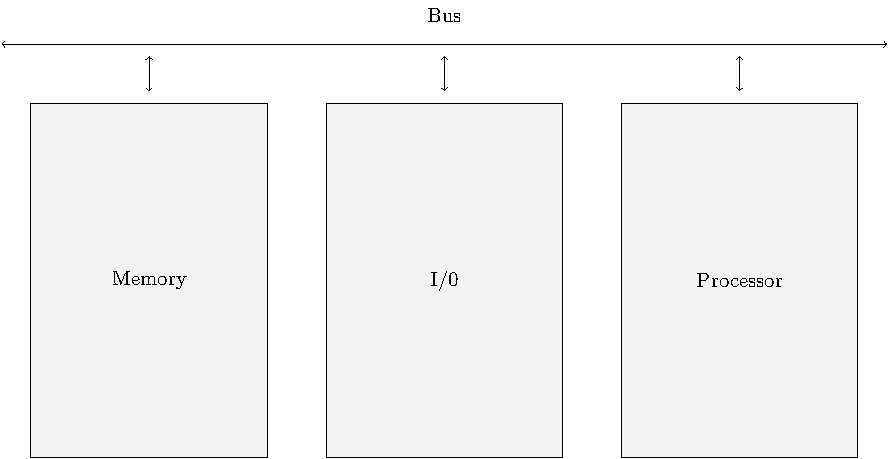
\includegraphics[width=90mm]{three_box_model.pdf}
	\caption{An example of the three box model}
	\label{overflow}
\end{figure}


\end{document}